%  LaTeX support: latex@mdpi.com 
%  For support, please attach all files needed for compiling as well as the log file, and specify your operating system, LaTeX version, and LaTeX editor.

%=================================================================
\documentclass[sensors,article,submit,oneauthor]{Definitions/mdpi} 
% For posting an early version of this manuscript as a preprint, you may use "preprints" as the journal. Changing "submit" to "accept" before posting will remove line numbers.

% Below journals will use APA reference format:
% admsci, aieduc, behavsci, businesses, econometrics, economies, education, ejihpe, famsci, games, humans, ijcs, ijfs, investment, fclam, jintelligence, journalmedia, jrfm, jsam, languages, opermanag, peacestud, pmh, psycholint, publications, tourismhosp, youth

% Below journals will use Chicago reference format:
% arts, genealogy, histories, humanities, laws, literature, religions, risks, socsci

%--------------------
% Class Options:
%--------------------
%----------
% journal
%----------
% Choose between the following MDPI journals:
% accountaudit, acn, acoustics, actuators, addictions, addictprev, adhesives, adolescents, aerobiology, aerospace, agriculture, agriengineering, agrochemicals, agronomy, ai, aichem, aieng, aimater, aimed, aipa, air, aisens, aisoc, algorithms, allergies, alloys, amh, analog, analytica, analytics, anatomia, anesthres, animals, antibiotics, antibodies, antioxidants, applbiosci, appliedchem, appliedmath, appliedphys, applmech, applmicrobiol, applnano, applsci, aps, aquacj, archaeolstud, architecture, arm, arthropoda, asc, asi, astronautics, astronomy, atmosphere, atoms, audiolres, automation, axioms, bacteria, batteries, bdcc, beverages, biochem, bioengineering, biologics, biology, biomass, biomechanics, biomed, biomedicines, biomedinformatics, biomimetics, biomolecules, biophysica, bioresourbioprod, biosensors, biosphere, biotech, birds, blockchains, bloods, blsf, brainsci, breath, buildings, cancers, carbon, cardio, cardiogenetics, cardiovascmed, catalysts, cells, ceramics, challenges, chemengineering, chemistry, chemosensors, chemproc, children, chips, cimb, civileng, cleantechnol, climate, clinbioenerg, clinpract, clockssleep, cmd, cmtr, coasts, coatings, colloids, colorants, commodities, complexities, complications, compounds, computation, computers, condensedmatter, conservation, constrmater, cosmetics, covid, crops, cryo, cryptography, crystals, csmf, ctn, culture, curroncol, cyber, dairy, data, ddc, dentistry, dermato, dermatopathology, designs, devices, dhi, diabetology, diagnostics, dietetics, digital, disabilities, diseases, diversity, dna, drones, drugreact, drylands, dynamics, earth, ebj, ecm, ecologies, edm, eesp, electricity, electrochem, electronicmat, electronics, embodiedintell, encyclopedia, endocrines, energies, eng, engproc, entomology, entropy, environments, environremediat, epidemiologia, epigenomes, esa, est, fermentation, fibers, fintech, fire, fishes, fluids, foodeng, foods, forecasting, forensicsci, forests, fossstud, foundations, fractalfract, freshwater, fuels, future, futureinternet, futurepharmacol, futurephys, futuretransp, galaxies, gases, gastroent, gastrointestdisord, gastronomy, gels, genes, geochem, geographies, geohazards, geomatics, geometry, geosciences, geotechnics, geriatrics, germs, glacies, grainsci, grasses, green, greenhealth, gucdd, gynecolcancer, hardware, hazardousmatters, healthcare, healthcmater, hearts, hemato, hematolrep, hep, heritage, higheredu, highthroughput, horticulturae, hospitals, hydrobiology, hydrogen, hydrology, hydrometeorology, hydropower, hygiene, idr, iic, ijem, ijerph, ijgi, ijmd, ijms, ijns, ijom, ijp, ijpb, ijt, ijtm, ijtpp, ijtst, ime, immuno, industries, inflammj, informatics, information, infrastructures, inorganics, insects, instruments, inventions, iot, j, jaestheticmed, jal, japma, jcdd, jcm, jcp, jcrm, jcs, jcto, jdad, jdb, jdream, jemr, jeta, jfb, jfmk, jfth, jgbg, jgg, jimaging, jlpea, jmahp, jmmp, jmms, jmp, jmse, jne, jnt, jof, joi, joitmc, joma, jop, joptm, jor, jox, jpbi, jphytomed, jpm, jsan, jtaer, jvd, jzbg, kidneydial, kinasesphosphatases, knowledge, labmed, laboratories, lam, land, lasers, legumes, life, lights, limnolrev, lipidology, liquids, livers, logics, logistics, lubricants, lymphatics, machines, macromol, magnetism, magnetochemistry, make, marinedrugs, maritime, materials, materproc, mathematics, mca, mcb, measurements, medicina, medicines, medsci, membranes, merits, metabolites, metals, meteorology, methane, metrics, metrology, micro, microarrays, microbiolres, microelectronics, micromachines, microorganisms, microplastics, microwave, minerals, mining, mmphys, modelling, molbank, molecules, mollusca, mps, msf, mti, multimedia, muscles, nanoenergyadv, nanomanufacturing, nanomaterials, ncrna, ndt, network, neuroglia, neuroimaging, neurolint, neurosci, nitrogen, notspecified, nursrep, nutraceuticals, nutrients, obesities, occuphealth, oceans, ohbm, onco, optics, oral, organics, organoids, osteology, oxygen, pandemics, parasites, parasitologia, particles, pathogens, pathophysiology, pediatrrep, pets, pharmaceuticals, pharmaceutics, pharmacoepidemiology, pharmacy, phc, philosophies, photochem, photonics, photovoltaics, phycology, physchem, physics, physiologia, plants, plasma, platforms, pollutants, polymers, polysaccharides, populations, poultry, powders, precision, precisoncol, preprints, proceedings, processes, prosthesis, proteomes, psf, psychiatryint, psychoactives, purification, quantumrep, quaternary, qubs, radiation, rareearths, rdt, reactions, realestate, receptors, recycling, regeneration, remotesensing, reports, reprodmed, resources, rheumato, rjpm, robotics, rsee, ruminants, safety, sanpp, sca, sci, scipharm, sclerosis, seeds, sensors, separations, sexes, shi, signals, sinusitis, siuj, skins, smartcities, smartfish, sna, societies, software, soilsystems, solar, solids, spectroscj, sports, standards, stats, std, stratsediment, stresses, strokerep, superintelligence, surfaces, surgeries, suschem, sustainability, sustainfoods, sustainpackag, symmetry, synbio, systems, tae, targets, taxonomy, technologies, telecom, test, textiles, thalassrep, therapeutics, thermo, timespace, tomography, toxics, toxins, tph, transplantology, transportation, traumacare, traumas, tri, tropicalmed, universe, urbansci, uro, vaccines, vehicles, venereology, vetsci, vibration, virtualworlds, viruses, vision, waste, water, welding, wem, wevj, wild, wind, women, world, zoonoticdis

%---------
% article
%---------
% The default type of manuscript is "article", but can be replaced by: 
% abstract, addendum, article, benchmark, book, bookreview, briefcommunication, briefreport, casereport, changes, clinicopathologicalchallenge, comment, commentary, communication, conceptpaper, conferenceproceedings, correction, conferencereport, creative, datadescriptor, discussion, entry, expressionofconcern, extendedabstract, editorial, essay, erratum, fieldguide, hypothesis, interestingimages, letter, meetingreport, monograph, newbookreceived, obituary, opinion, proceedingpaper, projectreport, reply, retraction, review, perspective, protocol, shortnote, studyprotocol, supfile, systematicreview, technicalnote, viewpoint, guidelines, registeredreport, tutorial,  giantsinurology, urologyaroundtheworld
% supfile = supplementary materials

%----------
% submit
%----------
% The class option "submit" will be changed to "accept" by the Editorial Office when the paper is accepted. This will only make changes to the frontpage (e.g., the logo of the journal will get visible), the headings, and the copyright information. Also, line numbering will be removed. Journal info and pagination for accepted papers will also be assigned by the Editorial Office.

%------------------
% moreauthors
%------------------
% If there is only one author the class option oneauthor should be used. Otherwise use the class option moreauthors.

%=================================================================
% MDPI internal commands - do not modify
\firstpage{1} 
\makeatletter 
\setcounter{page}{\@firstpage} 
\makeatother
\pubvolume{1}
\issuenum{1}
\articlenumber{0}
\pubyear{2026}
\copyrightyear{2026}
%\externaleditor{Firstname Lastname} % More than 1 editor, please add `` and '' before the last editor name
\datereceived{ } 
\daterevised{ } % Comment out if no revised date
\dateaccepted{ } 
\datepublished{ } 
%\datecorrected{} % For corrected papers: "Corrected: XXX" date in the original paper.
%\dateretracted{} % For retracted papers: "Retracted: XXX" date in the original paper.
%\doinum{} % Used for some special journals, like molbank
%\pdfoutput=1 % Uncommented for upload to arXiv.org
%\CorrStatement{yes}  % For updates
%\longauthorlist{yes} % For many authors that exceed the left citation part
%\IsAssociation{yes} % For association journals

%=================================================================
% Add packages and commands here. The following packages are loaded in our class file: fontenc, inputenc, calc, indentfirst, fancyhdr, graphicx, epstopdf, lastpage, ifthen, float, amsmath, amssymb, lineno, setspace, enumitem, mathpazo, booktabs, titlesec, etoolbox, tabto, xcolor, colortbl, soul, multirow, microtype, tikz, totcount, changepage, attrib, upgreek, array, tabularx, pbox, ragged2e, tocloft, marginnote, marginfix, enotez, amsthm, natbib, hyperref, cleveref, scrextend, url, geometry, newfloat, caption, draftwatermark, seqsplit
% cleveref: load \crefname definitions after \begin{document}

%=================================================================
% Please use the following mathematics environments: Theorem, Lemma, Corollary, Proposition, Characterization, Property, Problem, Example, ExamplesandDefinitions, Hypothesis, Remark, Definition, Notation, Assumption
%% For proofs, please use the proof environment (the amsthm package is loaded by the MDPI class).

%=================================================================

%--- Local adaptation: hide dates box, copyright box (left margin) ---
\makeatletter
\renewcommand{\leftcolDates}{}
\renewcommand{\leftcolumnCright}{}
\makeatother

\Title{Project Safe Wireless: Synthetic RSS/RTI Evaluation and a Separate CSI Presence Pilot}

\newcommand{\orcidauthorA}{}

\Author{Camilo Andr\'es V\'asquez Montenegro $^{1}$}

\AuthorNames{Camilo Andr\'es V\'asquez Montenegro}

\address{%
$^{1}$ \quad School of Mathematical and Computational Sciences, Yachay Tech University, Urcuqu\'i, Ecuador; camilo.vasquez@yachaytech.edu.ec}

\abstract{This revision examines two separate workstreams within Project Safe Wireless: synthetic received-signal-strength (RSS) radio tomographic imaging (RTI) for localization, and an exploratory physical channel-state-information (CSI) pilot for binary presence. Across two single-seed RTI configurations, the EM-derived Fisher method exactly matched an equivalent Tikhonov control. Its root-mean-square error (RMSE) was 4.015 m versus 4.113 m for Tikhonov in the 6-node pilot and 3.251 m versus 3.151 m in the 12-node configuration; constant-center predictions had RMSEs of 2.517 m and 2.650 m, respectively. A two-Gaussian mixture had slightly higher held-out residual log density than a single Gaussian in the short pilot ($-2.101$ versus $-2.145$), without establishing better localization. Separately, a 200-tree random forest evaluated by leaving one of three ESP32 acquisition rounds out scored 69.64\% balanced accuracy, F1 = 0.684, and a 27.38\% false-positive rate over 165 accepted two-second windows. User-confirmed labels, one environment, and variable fold performance limit this result. The evidence map has 1,413 records: 279 reviewed semantically and 1,134 pending. Existing RTI+EM and robust RTI precedents preclude a novelty claim. Per-link EM weighting under controlled missing measurements remains a proposed, untested next step. CSI presence, RTI localization, and single-link RSS acquisition are not fused or directly compared.}

\keyword{expectation-maximization; radio tomographic imaging; received signal strength; channel state information; ESP32; presence detection; missing measurements; reproducibility}

%=================================================================
\begin{document}

\newcolumntype{L}{>{\raggedright\arraybackslash}X}

\section{Introduction}

Device-free radio localization estimates an object's position without asking it to carry a transmitter. In RTI, changes in RSS across radio links are modelled as weighted contributions from cells in a spatial grid. The forward model is
\begin{equation}
\mathbf{y} = \mathbf{W}\mathbf{x} + \mathbf{n},
\end{equation}
where $\mathbf{y}$ contains the link measurements, $\mathbf{W}$ maps grid cells to links, $\mathbf{x}$ is the unknown attenuation field, and $\mathbf{n}$ is measurement noise. The number of links is often smaller than the number of cells, so the reconstruction is ill posed and needs regularization \cite{Wilson2010}.

The long-term motivation is to investigate radio-based sensing that could support the search for people under rubble. Prior rescue research has studied breathing-related motion with radar \cite{Takeuchi2008}. The present work is an initial computational step: it localizes an idealized attenuation target and leaves rubble and material properties outside the model. The simulation does not establish whether a person is present or whether radio sensing would work in a collapsed structure.

RTI estimates position from indirect RSS measurements, so its result depends on both the spatial model and the assumed noise. Expectation-Maximization (EM) can fit a two-component Gaussian mixture to RSS residuals, but a better statistical fit does not guarantee a more accurate position. The practical question is whether that improvement in noise modeling carries through to localization. Node geometry, regularization, calibration size, and target strength also affect the answer.

The objective of this study is to determine whether better statistical modelling of RSS noise leads to better position estimates, and by how much. From an AI standpoint, this is a question about unsupervised probabilistic modelling: whether a mixture model learned from unlabeled calibration residuals improves a downstream prediction.

This project tests that question under controlled synthetic conditions. EM estimates the mixture parameters and the latent component probabilities from calibration residuals; a separate validation block measures noise-model fit, and held-out test queries measure localization. The research question is: across the nine predefined synthetic scenarios, does a two-Gaussian mixture fitted by EM achieve higher held-out log density than a single Gaussian, and how does its Fisher-derived scaling affect localization error relative to standard Tikhonov RTI? What does the equivalent-regularization control reveal?

This study reports model fit and localization as separate outcomes and includes an equivalent-regularization control. The control tests whether the Fisher factor does more than rescale the Tikhonov penalty; in the present implementation, it does not. The current contribution is a reproducible preliminary comparison of these outcomes and a separate CSI presence pilot, not a new validated estimator. Because RSS/RTI with EM already has direct precedent, any methodological contribution must be tied to a specific formulation and tested against appropriate controls and prior methods \cite{Wilson2010,Kaltiokallio2021,Huang2020}.

This V3 revision continues the V1 synthetic RTI study and the V2 propagation and CSI work. Its first question is whether the existing EM-derived scaling changes synthetic RTI localization after controlling for equivalent regularization. Its second, separate question is how a small physical CSI model behaves on complete held-out acquisition rounds. These branches are not fused: CSI classification metrics do not measure RTI localization, and the single-link Windows RSS capture does not form a tomographic image. A future rescue application remains a motivation, not a result of this study.
\section{Related Work}

Dempster, Laird, and Rubin described EM as a general maximum-likelihood method for models with incomplete data, including finite mixtures \cite{Dempster1977}. Wu later analysed when EM sequences converge \cite{Wu1983}. In practice, reaching the iteration limit or returning a stable parameter vector does not establish that the fitted model suits the data or improves a downstream prediction.

Wilson and Patwari introduced a linear RSS-based RTI model and used Tikhonov regularization to reconstruct attenuation images \cite{Wilson2010}. They also fitted a two-component Gaussian mixture to measured RSS residuals with EM. The base simulation uses their reported values, $p=0.548$, $\sigma_1=0.971$~dB, and $\sigma_2=3.003$~dB, as fixed generator settings. This project does not measure those parameters. Their experiment used IEEE 802.15.4 sensor nodes, so its measurements are not a Wi-Fi dataset.

These RTI and noise parameters \cite{Wilson2010}, the general EM formulation \cite{Dempster1977}, and the convergence analysis \cite{Wu1983} are the three main scientific foundations of the present implementation. Other studies below inform its comparisons and future direction.

Later RTI studies combined mixture models with reconstruction methods. Gao et al. used a Gaussian mixture model and matrix-transform restoration, and evaluated it with simulated and experimental targets \cite{Gao2017}. Huang and Yang estimated mixture-noise parameters and the attenuation image together through sparse Bayesian learning (SBL) \cite{Huang2020}. Zhao and Patwari addressed a related problem in variance-based device-free localization: they either projected the measurements away from a noise subspace learned from calibration data or weighted them with an estimated link-noise covariance, and reported lower localization RMSE than the standard Tikhonov-based estimator in two measured experiments \cite{Zhao2011}. In this implementation, the Fisher term is one scalar that changes the Tikhonov regularization. It does not assign different noise weights to individual links, as a link-adaptive estimator would.

Kaltiokallio et al. used EM with Gaussian smoothing to learn RSS model parameters for device-free localization and tracking, then evaluated the method on measured data from two environments \cite{Kaltiokallio2021}. Their experiments track moving targets; this project uses static synthetic queries on one grid. RADAR provides an earlier example of RF localization from signal strengths and known locations \cite{Bahl2000}. The K-NN method here is a weighted fingerprint baseline with synthetic data, rather than a reproduction of RADAR.

For the intended rescue context, Takeuchi et al. studied a radar system that used breathing-related motion to locate survivors under rubble \cite{Takeuchi2008}. Its sensing modality and experimental setting differ from the RSS-based synthetic localization studied here. The software also draws on IsukaW's Wi-Fi sensing repository \cite{IsukaW}: the current project reuses its WiFiMeasurement data contract, while the synthetic generator, EM calibration, and RTI evaluation form a separate integration. The repository is cited as software provenance, not as experimental evidence for rescue performance. Table~\ref{tab:related} summarizes the related studies.

The extension distinguishes activity from presence. CARM connects CSI dynamics to activity recognition and reports an average accuracy above 96\% in its experiments \cite{Wang2015CARM}; this is not stationary-presence accuracy. Liu et al.\ combine CSI magnitude and phase CNN branches with temporal post-processing \cite{Liu2022Presence}. Their author manuscript reports collection on 24 days in three environments, but states that complete stillness is likely classified as no motion before post-processing. Neither validates our ESP32 hardware or still-person protocol, and their scores are not transferred to this study.

IsukaW remains software provenance rather than a performance benchmark. The remote audit resolved revision \texttt{91aee04ea938274d014a3981d409f83267ea15c0}; an earlier local copy was \texttt{065c12be3b0fb34d458d74d36d3534746e285f84}. Its Wi-Fi path uses RSSI and heuristic radar coordinates; CSI is declared but no connected collector was identified. Camera-assisted fusion supplies an additional modality. RTI/EM belong to Project Safe Wireless, not that reference. No measured performance ranking against it is claimed.

\begin{table}[H]
\caption{Summary of related work.\label{tab:related}}
\begin{adjustwidth}{-\extralength}{0cm}
\scriptsize
\setlength{\tabcolsep}{3pt}
\begin{tabularx}{\fulllength}{>{\raggedright\arraybackslash}p{1.6cm}LLLLLL}
\toprule
\textbf{Reference} & \textbf{Main Idea / Problem} & \textbf{Model / Algorithm} & \textbf{Dataset} & \textbf{Metric(s)} & \textbf{Main Result(s)} & \textbf{Limitation(s)}\\
\midrule
Wilson \& Patwari \cite{Wilson2010} & Infer attenuation images from RSS changes across links. & Linear RTI weights, Tikhonov reconstruction, and EM fit of two-Gaussian RSS noise. & Deployed 28-node sensor network over 441~ft$^2$. & Image MSE and geometry-based MSE bounds. & Demonstrates RTI reconstruction with measured RSS; accuracy depends on geometry and parameter choice. & IEEE 802.15.4 deployment; it does not isolate EM's effect on downstream position error.\\
\addlinespace
Gao et al. \cite{Gao2017} & Restore blurred RTI images to recover target shape. & Gaussian-mixture degradation model, matrix transform, constrained least-squares filter. & Simulated target shapes and an indoor RTI experiment. & Image MSE, edge-preservation index, and SSIM. & Reports improved target detail and image-quality measures over shadowing-based RTI. & Focuses on image restoration, not noise calibration or position-error gains.\\
\addlinespace
Huang \& Yang \cite{Huang2020} & Reduce mislocalization under complex, non-Gaussian RTI noise. & Sparse Bayesian learning jointly estimates a Gaussian-mixture noise model and attenuation image. & 20-node, 6~m $\times$ 4~m setup; predefined single- and multi-target positions. & Mean and maximum localization error; multi-target set-distance. & SBL-NA outperformed Tikhonov, BCS, HBCS, and Laplace baselines in reported localization errors; best tested mixture used $K=3$. & Joint SBL reconstruction is more complex and differs from this study's two-Gaussian calibration control.\\
\addlinespace
Zhao \& Patwari \cite{Zhao2011} & Reduce the effect of intrinsic motion noise (e.g., wind) in variance-based device-free localization. & Variance-based RTI with a subspace projection (SubVRT) or covariance-weighted least squares (LSVRT). & 34 TelosB nodes and 1122 links around a house; two measured experiments (calm and windy). & Localization and tracking RMSE. & Windy case: RMSE 1.26~m (VRTI) versus 0.74~m (SubVRT) and 0.69~m (LSVRT); small gains in the calm case. & Detects motion rather than static attenuation; LSVRT assumes Gaussian noise; needs calibration data.\\
\addlinespace
Kaltiokallio et al. \cite{Kaltiokallio2021} & Learn RSS parameters online while tracking device-free targets. & Gaussian smoothing with EM and Bayesian filtering with measurement selection. & 18 experiments in a 75~m$^2$ open area and an 82~m$^2$ apartment. & Tracking RMSE and computation time. & Reports 17~cm and 37~cm tracking accuracy; 42\% lower RMSE than ARTI and EM up to 18$\times$ faster than nonlinear optimization. & Dynamic measured-RSS tracking, not static synthetic RTI localization.\\
\addlinespace
Bahl \& Padmanabhan \cite{Bahl2000} & Locate building occupants from WLAN signal strengths. & Empirical nearest-neighbor fingerprints and a propagation-model baseline. & Indoor WLAN deployment with three base stations and known-location samples. & Percentile and median position error. & Reports a 2--3~m median for empirical fingerprints, versus 4.3~m for propagation modeling. & Site-specific calibration; older WLAN setup; no tomography or EM noise estimation.\\
\addlinespace
Takeuchi et al. \cite{Takeuchi2008} & Detect breathing motion to locate survivors under rubble. & Pulse-Doppler rescue radar with a two-dimensional array and 3D location estimation. & Experimental rescue-radar evaluation; the article abstract does not give a sample count. & Experimental feasibility of 3D survivor localization; not directly comparable to RSS RMSE. & The authors report experimental assessment of the array-based approach. & Different sensing modality and target signal; motivation only, not an RTI benchmark.\\
\addlinespace
Wang et al.\ \cite{Wang2015CARM} & Relate CSI dynamics to activities. & CSI--speed and CSI--activity models (CARM). & Commercial Wi-Fi in multiple environments; counts not reconciled here. & Activity accuracy. & Reports average accuracy above 96\%. & Activity recognition does not establish still presence or ESP32 performance.\\
\addlinespace
Liu et al.\ \cite{Liu2022Presence} & Presence from ambient Wi-Fi. & Magnitude/phase CNN and temporal post-processing. & Atheros CSI; 24 days, three environments, eight months. & Motion/presence tests; false-positive duration. & Four false-positive seconds in about 46.5 h of human-free test. & Completely still persons may be negative for the motion model; hardware/protocol differ.\\
\bottomrule
\end{tabularx}
\end{adjustwidth}
\end{table}

Kaltiokallio et al. provide a direct RSS/EM localization and tracking precedent. Their measured network used 20 TI CC2531 nodes at 2.4 GHz IEEE 802.15.4, with RSS links, RTI-based position estimates, Bayesian filtering and smoothing; EM updated per-link RSS-model parameters and variance. This is not Wi-Fi or ESP32, and its principal outcomes are tracking/localization rather than binary presence. It means that using RSS, RTI and EM together is not itself a novel claim \cite{Kaltiokallio2021}.

A distinct robust-RTI precedent is Wang et al., who use sparse Bayesian learning (SBL) with a Laplace prior to reduce image artifacts from multipath fading. In one through-wall scenario they report a mean localization error of 0.43 m for Laplace, compared with 0.70 m for a Jeffrey prior and 0.88 m for Student-t. This addresses spatial sparsity and multipath; it is not the EM method studied here and does not establish robustness to missing RSS packets \cite{Wang2019Laplace}. De Alwis et al. use packet-loss ratio itself as the RTI observation. That is different from a conventional RSS-RTI system in which a lost packet removes an RSS measurement and must be represented as missing, not as zero RSS \cite{DeAlwis2016}.

CSI-based presence and activity are another, separate branch. Strohmayer and Kampel classify ESP32 CSI spectrograms in a through-wall setup; their task and input differ from an RSS attenuation image \cite{Strohmayer2023ESP32}. The public CSI-GaitCov release targets gait-based person identification across walking direction and backpack conditions, not empty-versus-present detection or RTI localization; it is not used in the reported model \cite{GaitCov2026}. These examples motivate keeping presence, activity, identity, image reconstruction and position estimation as separate outcomes.

Human-body shadowing studies also do not support a universal person-specific dB threshold. At 2.4 GHz, Januszkiewicz reports a median path-loss increase from 53 to 63 dB for one measured geometry with a person in the link path, while another geometry with two people near the transmitter changed the median from 53 to 54 dB. These are geometry-specific results, not a general signature that distinguishes a person from a wall \cite{Januszkiewicz2018}.

\section{Materials and Methods}

\subsection{Study Design and Data Generation}

V3 reports two distinct workstreams: a synthetic RSS/RTI localization experiment inherited from V1, and a physical ESP32 CSI presence pilot added in V2. Their acquisition, algorithms, partitions and metrics remain separate; no fusion model was evaluated.

The V1 layer is a fundamental-research study: it investigates whether an EM-fitted noise model improves a standard RTI algorithm, rather than solving a deployed application. It is an in silico study using simulated measurements. The generator places radio nodes around a rectangular area, builds the ellipse-based weight matrix $\mathbf{W}$, draws one target attenuation field $\mathbf{x}$, and generates link changes using $\mathbf{y}=\mathbf{W}\mathbf{x}+\mathbf{n}$. It records RSS as the reference level minus the generated attenuation. Each CSV row identifies its link and data phase; missing measurements are marked explicitly, and the target position is saved separately as ground truth.

The base mixture uses Wilson and Patwari's published values \cite{Wilson2010}. The quick run has six nodes, 15 links, 36 grid cells, and 30 test queries. The larger base run uses 12 nodes, 66 links, 100 cells, and 120 test queries. Both configurations save separate reference, calibration, validation, fingerprint, development, and test data. The simulator can vary noise spread, quantization, temporal correlation, link loss, baseline drift, carrier frequency, and receiver margin. In this model, carrier frequency changes the illustrative free-space link budget and which weak links are censored; it does not change the spatial weight matrix or simulate signal penetration through materials.

The system workflow (Figure~\ref{fig:workflow}) connects synthetic data generation, EM noise calibration, held-out noise validation, localization, and evaluation. Known fingerprint positions are used by K-NN and development positions select hyperparameters; the true positions of test queries are reserved for final evaluation.

\begin{figure}[H]
\centering
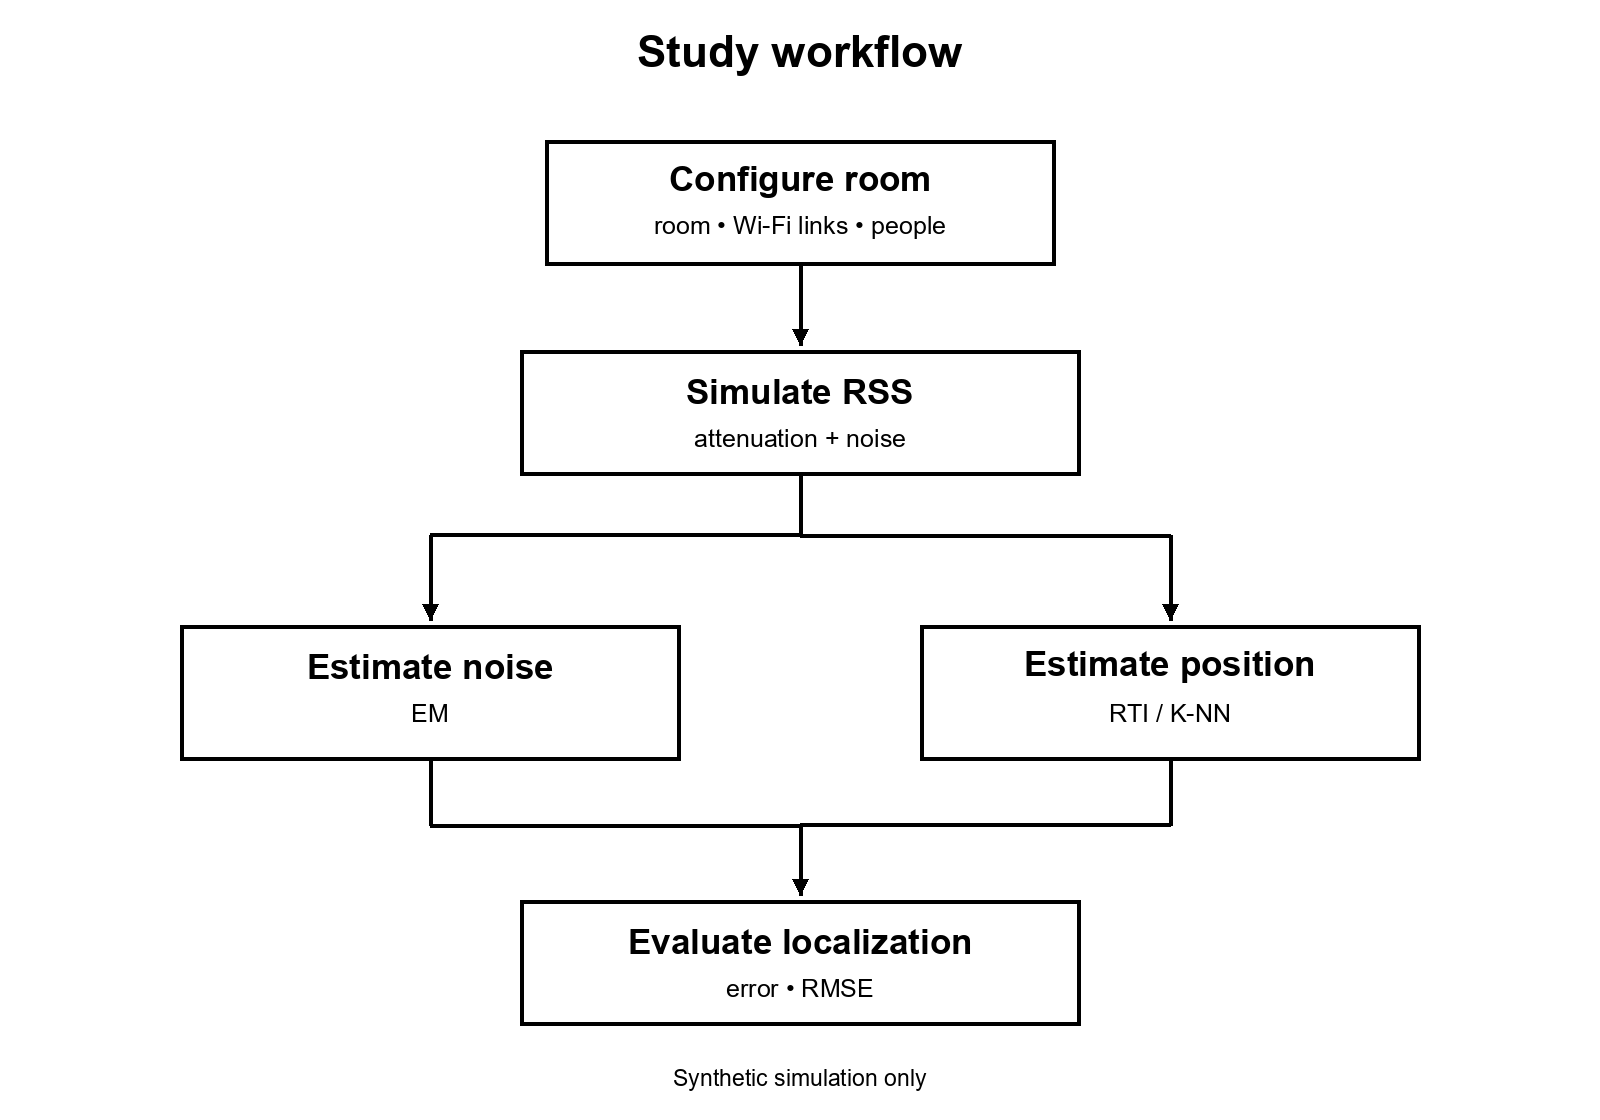
\includegraphics[width=10.5cm]{fig1.png}
\caption{Study workflow. The simulated room, links, and people are configured; RSS is simulated with attenuation and noise; EM estimates the noise model while RTI or K-NN estimates position; both feed the evaluation of localization error and RMSE. Synthetic simulation only.\label{fig:workflow}}
\end{figure}
\unskip

The V1 design is retained as the synthetic RTI layer. The new propagation layer uses Sionna RT 1.2.2, Mitsuba 3.8.0 and Dr.Jit 1.3.1 \cite{SionnaRT122}. It calculates paths, CIR, CFR and radio maps; local checks include LoS/Friis and absolute delay. Two static channels are adapted to an array of shape $(1,64,10)$ with no class prediction. These ideal frequency bins are not chipset CSI. Observation noise does not create gait or respiration, and bodies/materials remain illustrative. A Windows \texttt{LIVE\_RSSI} observation with system-reported dBm verifies intensity acquisition only. RF interference and quantitative low/medium noise profiles remain unvalidated.

A separate \texttt{SYNTHETIC (fake)} development source produced 240 designed windows in four classes and three arbitrary domains called rooms. They are neither measured rooms nor Sionna scenes. This source supplies numerical and grouped-evaluation software controls, not physical classification evidence.

Physical acquisition used ESP32-D0WD-V3 revision v3.1, ESP-IDF v6.1 and the official \texttt{esp-csi} router example at commit \texttt{8633d67152db2808f141cc1595970aa9cf406045}, with a documented local compatibility patch \cite{EspCSI2026}. The first unlabeled check retained 4,985 valid packets in 30.032 s. Packet times were irregular. The four initial bytes marked invalid were preserved raw and excluded from analysis; no physical subcarrier frequencies were assigned to payload indices.

Figure~\ref{fig:workflow} is the original student-designed Figma diagram documented in V1 and is retained unchanged. It represents the synthetic workflow. The course requires the system diagram to be designed by the student, not generated by AI \cite{CourseRubric2026}. The student must update it to cover the CSI extension before claiming it depicts the complete V2 system; a measured-results plot is not a substitute.

\subsection{Evidence Map and Acquisition Boundaries}

The literature inventory was assembled from the available bibliographic exports and deduplicated before screening. It contains 1,413 working records: 1,410 groups from eight CSV exports, one added DFLT--EM seed study, and two supplementary PDF records. Semantic review is incomplete (279 reviewed; 1,134 automatic proposals pending manual screening), and exports from Scopus and Web of Science were not authenticated. This inventory supports an exploratory, targeted synthesis only; it is not a systematic review and cannot establish absence of prior work.

A separate physical RSS acquisition check used a Windows laptop connected to one 2.4-GHz router link. The logger queried the Windows WLAN interface at approximately 1-s intervals, stored driver-reported RSSI in dBm, and retained signal quality as a separate percentage without converting it to dBm. These local captures were not used to estimate detection accuracy: a single link cannot form RTI, the labels and trial exclusions were not independently verified, and no matched multi-link reference was available.

The 14.4-GB CSI-GaitCov archive was downloaded and extracted, but no analysis of it was completed for this revision. It is a gait-identification dataset with walking-direction and backpack covariates, not a labeled empty/presence set for this study; it contributes no result to this manuscript \cite{GaitCov2026}.
\subsection{Inputs, Partitions, and Algorithms}

The estimator receives calibration residuals after the reference estimate has been subtracted. The C++17 EM code estimates the mixture weight $p$ and both standard deviations while holding the component means at zero. A separate validation block compares the fitted mixture's average held-out log density with that of a single Gaussian. This measures how well each distribution predicts residuals; it does not measure localization accuracy.

The generator uses separate random streams for reference, calibration, noise validation, fingerprints, development, and test data. Development data selects regularization $\alpha$ and $K$; test data is reserved for scoring. K-NN fingerprints cover the same grid as the test locations but have independent noise draws. The current experiment therefore tests localization within a known grid. It does not test unseen positions, moving trajectories, multiple targets, or transfer to a different environment.

The localization comparison includes five methods: (1) Tikhonov RTI, (2) RTI with a Fisher factor calculated from the EM mixture, (3) a Tikhonov control with the equivalent regularization, (4) inverse-distance weighted K-NN on synthetic fingerprints, and (5) a constant prediction at the room center. In this implementation, the Fisher factor only rescales the Tikhonov penalty. The matched control checks that algebra; the equality does not demonstrate link-specific noise handling.

The physical pilot acquired three rounds, each with a separate operational empty reference, then empty, walking, still and final-empty recordings. Conditions were confirmed by the student, without external verification of labels, positions or distances. A previously fixed packet format was used. Amplitudes were normalized to the median empty reference. Two-second windows were resampled to 50 Hz from actual times without extrapolation or gaps over 100 ms. Calibration windows were not scored as empty examples.

The physical classifier uses twelve summaries of log amplitude ratios, static profiles and temporal variation. Settings were fixed at 200 trees, maximum depth 5, minimum leaf size 3, balanced class weights, seed 0, one worker and threshold 0.5. Each of three folds fits two complete rounds and holds out the third. That round uses its own separate empty reference: this is evaluation after environmental calibration, not transfer without a reference. Forest votes are uncalibrated scores. The artificial four-class control is different: separate synthetic rooms fit the forest, calibrate a sigmoid and test.

\subsection{Metrics and Planned Experiments}

For noise fit, the study records EM convergence, estimated parameters, and mean held-out log density (natural log per residual; residuals are in dB). For localization, it reports mean Euclidean error, RMSE in meters, and coverage. Mean, median, and RMS position error are the metrics reported by the RTI and RF-localization studies reviewed above \cite{Huang2020,Zhao2011,Kaltiokallio2021,Bahl2000}, and the held-out log density measures how well a fitted distribution predicts unseen residuals. The saved tables identify missing predictions and any center fallback. The V1 synthetic pilot uses one seed. The final evaluation will repeat the base and stress scenarios with independent seeds, summarize variation across runs, and compare methods on the same test queries.

The next stage will first reproduce the nine-scenario pilot, then repeat it across seeds to measure variability and convergence. The larger base geometry will also be run with several seeds. Correlated-noise and low-margin cases will be reported as failures or insufficient calibration whenever the estimator cannot fit the data. Each run saves its configuration, code hashes, generated CSVs, predictions, and summary. The main pipeline uses Python, NumPy, Matplotlib, and the existing C++17 EM code. Optional pandas and SciPy are only needed for diagnostics adapted from the upstream repository.

The next work is ordered by research dependency rather than calendar dates. The proposed phases below are plans, not completed experiments.

\begin{table}[H]
\caption{Proposed research phases after the presentation.\label{tab:schedule}}
\begin{tabularx}{\textwidth}{>{\centering\arraybackslash}p{1.8cm}LL}
\toprule
\textbf{Phase} & \textbf{Work} & \textbf{Deliverable}\\
\midrule
1. Evidence & Complete manual screening of the 1,134 pending records and verify the prioritized full texts. & Updated source matrix and a bounded novelty statement.\\
2. Simulation & Specify the EM-weighted RTI candidate; compare it with Tikhonov, SBL--Laplace, matched Fisher, K-NN and center controls under identical data and masks. & Reproducible results across predeclared seeds, noise conditions and packet-outage patterns.\\
3. Physical RSS & Build a fixed multi-link layout with crossing paths, empty references and independently recorded positions; test calibration and missing-link handling. & Link-level measurements suitable for RTI, with session-separated evaluation.\\
4. CSI presence & Analyze CSI-GaitCov only for its supported gait/identity task; separately collect empty, still and moving presence sessions for presence evaluation. & Task-specific metrics with frozen models and held-out sessions.\\
5. Rescue & Consider obstructed or rubble-like conditions only after controlled localization and presence tests are reproducible. & A later, separately validated rescue-sensing study.\\
\bottomrule
\end{tabularx}
\end{table}

Presence outcomes remain PPV, recall, F1, balanced accuracy, false-positive rate and latency; spatial outcomes remain localization error and image quality. They answer different questions and are not pooled into a single improvement score.
\subsection{Baselines and Validity Checks}

Tikhonov RTI is the main algorithmic baseline, following the foundational RTI formulation \cite{Wilson2010}. Its equivalent-regularization control checks whether the Fisher factor does anything beyond changing the penalty strength. Weighted K-NN provides a fingerprint comparison inspired by RF location systems \cite{Bahl2000}, and the room-center prediction checks whether the signal-based methods improve on a simple spatial prior. Calibration and validation data are disjoint. Hyperparameters are selected with development data and are fixed before test scoring.

The simulator also checks that CSV values survive a write-read cycle, link identities remain consistent, missing values stay marked, and each run records its parameter sources. Correlated noise violates the independence assumption of the base mixture model, and EM may fail to converge under that condition. When a low receiver margin leaves too few calibration residuals, the run stops before fitting. In either case, the summary reports the failure or insufficient calibration and omits a localization score when the pipeline cannot validly produce one.

For the new applied task, two simpler baselines were evaluated on exactly the same 165 accepted windows, twelve features, empty references and three held-out-round partitions. The majority classifier learns its class from training only, with class zero in a tie. Logistic regression uses a training-only \texttt{StandardScaler} pipeline, $C=1$, L2 regularization, \texttt{lbfgs}, balanced weights, tolerance $10^{-4}$ and at most 1,000 iterations. Threshold 0.5 was fixed; no hyperparameter/threshold search used test results. The original forest exactly reproduced its saved provenance, indices, scores, predictions and metrics. The baselines were added after inspecting the forest, so the comparison is exploratory; it does not compare CSI with RSSI/RTI or camera-assisted IsukaW.

Physical checks preserve hashes, distinct files, non-overlapping acquisition intervals and intact rounds. They do not establish independent persons or replicates. Rejected windows are not absence predictions. No intervals assume 165 independent observations. Editor actors remain known geometry, not inferred species, counts or positions.

\subsection{Reproducibility}

\begingroup\sloppy\emergencystretch=2em
The project repository (\url{https://github.com/Camimilo-11/Ai-Yachay-2026/tree/main/Project-safe-wireless}) holds the simulator, the EM calibration code, the evaluation scripts, the run configurations with seeds and code hashes, the raw synthetic data, a requirements file, and the generated predictions, summaries, and figures. A verification script checks the package; one command (\texttt{ejecutar\_integracion.py -{}-quick -{}-suite}) runs the nine short scenarios, and a second command with the base configuration runs the full 12-node, 100-cell setup. Each run writes to a new output folder, and the README documents the steps. The required software is Python 3.10 or later and a C++17 compiler (g++); the Python scripts are the reproduction workflow, so no notebook is needed. All V1 data are synthetic; the measured extension is separate and its raw radio identifiers remain local.\par\endgroup

\begingroup\sloppy\emergencystretch=2em
The original RTI/EM project structure is retained. The measured extension currently resides in the local \texttt{safe-wirreles} working copy; integration and synchronization with the linked academic repository remain pending. The legacy environment requires Python 3.10 or later and C++17; the Sionna extension uses its separate pinned Python 3.12 environment. Commands and result paths below are relative to the extension root. This avoids mixing incompatible environment assumptions.

The extension preserves firmware/data hashes, manifests, JSON models, window quality and fold predictions. Summaries are \path{results/esp32/presence-model-20261030.json} and \path{results/esp32/presence-baselines-20261030.json}. The original model summary identifies commit \texttt{\seqsplit{544fe3f33ab97b7cecdf80da82d9f03d7de4063b}}.

The public derived dataset \path{results/esp32/public-presence-features-20261030.npz} contains exactly 165 rows and twelve numeric features, labels, anonymous round codes and conditions, with a JSON metadata companion. The reproduction command is \path{scripts/reproduce_presence_from_features.py}; it re-fits the forest and both baselines on the preserved folds and checks exact scores, predictions and metrics. This permits evaluation reproduction without raw network identifiers. It does not independently reproduce packet parsing, filtering, empty calibration, interpolation or feature extraction; those stages require the retained private raw files and manifests. Public metadata explicitly distinguishes redacted provenance from the private manifest. The original synthetic data and measured derived data remain separate.
\par\endgroup

\begin{quote}\small
\begin{verbatim}
# From the local safe-wirreles extension root:
$repro = @(
  "scripts/reproduce_presence_from_features.py"
  "--dataset"
  "results/esp32/public-presence-features-20261030.npz"
  "--metadata"
  "results/esp32/public-presence-features-20261030.json"
  "--output"
  "output/public-presence-reproduction.json"
)
.\.venv\Scripts\python.exe @repro
\end{verbatim}
\end{quote}

\section{Preliminary Results}

The quick base run used seed 7, six nodes, 15 links, 36 cells, and 30 test queries. EM converged after 294 iterations using 900 calibration residuals. It estimated $\hat{p}=0.541$, $\hat{\sigma}_1=1.060$~dB, and $\hat{\sigma}_2=2.938$~dB. For 450 held-out residuals, the mixture's mean log density was $-2.101$; the single Gaussian's was $-2.145$. The difference is small and comes from one generated split. Table~\ref{tab:results} reports the localization results.

\begin{table}[H]
\caption{Localization results of the quick base run (seed 7, 30 test queries).\label{tab:results}}
\begin{tabularx}{\textwidth}{>{\raggedright\arraybackslash}XCCC}
\toprule
\textbf{Method} & \textbf{Mean Localization Error (m)} & \textbf{RMSE (m)} & \textbf{Coverage}\\
\midrule
Tikhonov RTI & 3.653 & 4.113 & 30/30\\
EM-derived Fisher RTI & 3.530 & 4.015 & 30/30\\
Matched Tikhonov & 3.530 & 4.015 & 30/30\\
Weighted K-NN & 2.529 & 2.836 & 30/30\\
Constant room center & 2.357 & 2.517 & 30/30\\
\bottomrule
\end{tabularx}
\end{table}

The center prediction has the lowest mean error in the 6-node pilot, while K-NN performs better than either RTI setting. In the 12-node configuration, the center also has the lowest RMSE. The Fisher-based RTI and its equivalent Tikhonov control agree to numerical precision, as expected from the equations. Across the nine single-seed stress scenarios, seven returned status \texttt{ok}; EM did not converge within 600 iterations at temporal correlation $\rho=0.8$, and a 5-GHz low-margin run had only 1.3\% of test measurements available and insufficient calibration. The artificial packet-loss condition was a single simulated run, not a repeated robustness evaluation. None of these values is a measured Wi-Fi channel result.
The files under \texttt{results/integracion\_verificada/} contain the reported values. The table uses \texttt{base\_r00/summary.json} and can be regenerated with the command in the README. This is an executed simulation with one seed; it is not a physical experiment.

The larger V1 base configuration was also preserved: twelve nodes, 66 links, 100 cells and 120 test queries. Mean errors were 2.333 m for Tikhonov, 2.433 m for Fisher RTI and its matched control, 2.408 m for K-NN, and 2.483 m for the center. The corresponding RMSE values were 3.151, 3.251, 3.251, 2.677 and 2.650 m. Geometry and sample size differ from the quick pilot and are not pooled. An older 500-query audit does not replace either canonical V1 result.

The artificial CSI ablation gave macro F1 0.9143 for signal and signal plus material descriptors. Brier changed from 0.1062 to 0.1056, while \texttt{other\_moving} predicted as \texttt{human} increased from 0/60 to 20/60. This adverse result is preserved without claiming improvement. An initial physical empty/walking pair showed a 20.94\% increase in median within-second RMS-amplitude coefficient of variation, with overlapping distributions: a descriptive contrast, not classification accuracy.

The physical model accepted 165 of 183 windows: twelve were rejected for gaps and six for boundary coverage. There were 84 empty and 81 person-present windows (42 still, 39 walking), from three rounds in one campaign; these are not 165 persons or independent experiments. Table~\ref{tab:csi-baselines} compares models on identical accepted windows.

\begin{table}[H]
\caption{Exploratory physical CSI comparison using the same held-out-round predictions. Percentages except F1. PPV is undefined without positive predictions.\label{tab:csi-baselines}}
\scriptsize
\begin{tabularx}{\textwidth}{LCCCCCC}
\toprule
\textbf{Model} & \textbf{PPV (\%)} & \textbf{Recall (\%)} & \textbf{F1} & \textbf{BA (\%)} & \textbf{FPR (\%)} & \textbf{Still recall (\%)}\\
\midrule
Random forest & 70.13 & 66.67 & 0.6835 & 69.64 & 27.38 & 61.90\\
Logistic regression & 59.78 & 67.90 & 0.6358 & 61.93 & 44.05 & 66.67\\
Training majority & Undefined & 0.00 & 0.0000 & 50.00 & 0.00 & 0.00\\
\bottomrule
\end{tabularx}
\end{table}

Forest counts were TN=61, FP=23, FN=27 and TP=54; logistic regression gave TN=47, FP=37, FN=26 and TP=55; majority gave TN=84, FP=0, FN=81 and TP=0. Walking sensitivity was 71.79\% for the forest and 69.23\% for logistic regression. Forest still-person sensitivity was 0\%, 100\% and 85.71\% across rounds. The first fold's 100\% PPV means only two correct alerts alongside 25 false negatives. The exported forest was later fitted on all three rounds; the evaluation forests fit two. A functional prediction check on training data was excluded from evaluation.

\begin{figure}[H]
\centering
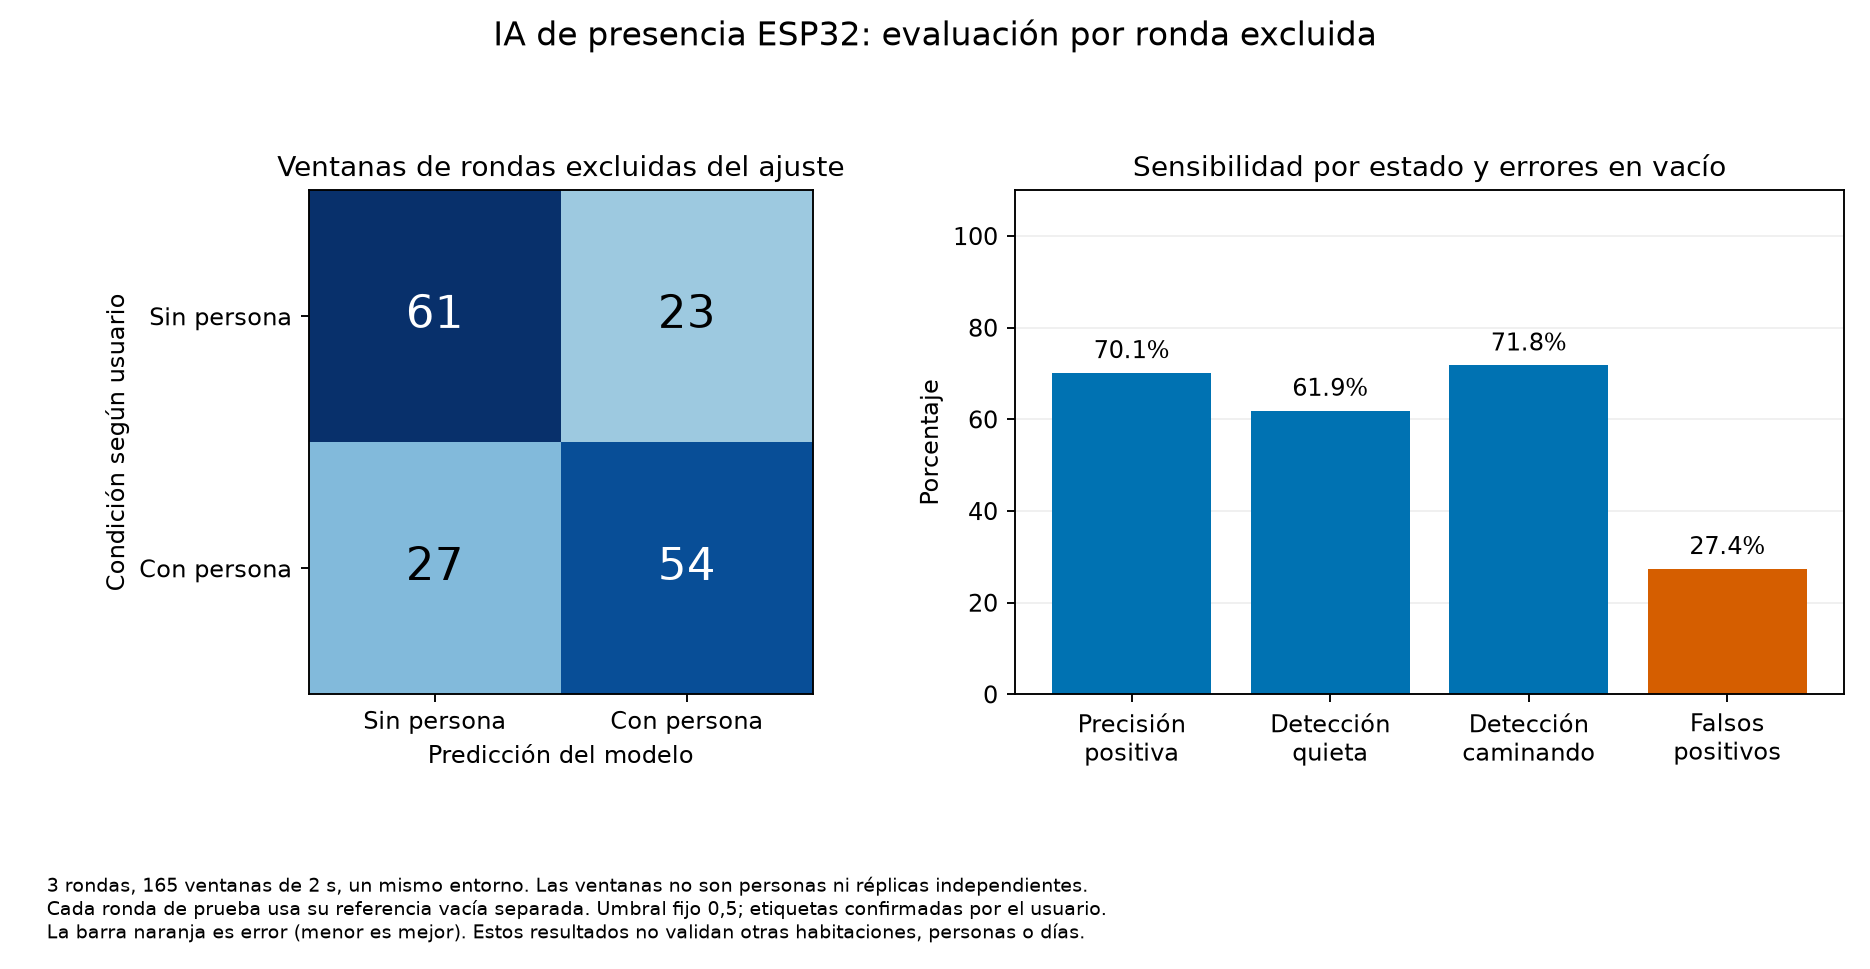
\includegraphics[width=\textwidth]{presence-model-20261030.png}
\caption{Physical CSI pilot. Left: reference rows and predicted columns. Right: forest PPV, still/walking sensitivity and empty-condition false positives (orange). There are 165 valid two-second windows from three rounds in one environment, each with its own separate empty reference. Windows are not independent persons. This results plot does not replace the student-designed system diagram.\label{fig:csi-pilot}}
\end{figure}

\section{Discussion and Expected Research Direction}

The two synthetic base configurations do not show an independent localization benefit from the current EM-derived Fisher factor. In the 6-node pilot it has lower RMSE than standard Tikhonov, but exactly matches the Tikhonov control with equivalent regularization; in the 12-node configuration its RMSE is higher than standard Tikhonov. The constant room-center prediction has the lowest RMSE in both configurations. The mixture's slightly higher held-out residual log density in the short pilot is a noise-fit result, not evidence of better localization. Each canonical base result uses one seed, so the differences do not estimate variability or generalize beyond these simulated settings.

The nine-run stress suite is also exploratory. Seven runs completed, one correlated-noise run did not converge within the preset iteration limit, and one 5-GHz low-margin run had insufficient calibration. The simulated packet-loss case is only one run and is not a robustness curve. Carrier frequency in this model changes an illustrative free-space link budget and censoring; it does not model material penetration, multipath or IEEE 802.11 packet behavior. The synthetic CSI and Sionna controls likewise do not supply measured human-body propagation. Their results must not be read as physical performance. In the artificial four-class CSI ablation, adding material descriptors left macro F1 at 0.9143 and changed Brier score from 0.1062 to 0.1056, while errors for the other-moving class increased from 0/60 to 20/60; these designed controls do not establish a physical classification gain.

The literature already contains RSS/RTI with EM for device-free localization and tracking, and separate RTI methods for multipath robustness. The defensible open question is narrower: whether a specific EM-derived, per-link reliability term improves RTI inversion when noise and missing RSS observations are controlled independently. One candidate is to compute a posterior responsibility $\gamma_i$ for the low-variance mixture component for each observed link residual and form
\begin{equation}
w_i = \frac{\gamma_i}{\sigma_1^2}+\frac{1-\gamma_i}{\sigma_2^2}, \qquad i\in\Omega,
\end{equation}
then alternate that weighting with a regularized inverse step,
\begin{equation}
\widehat{\mathbf{x}}=\arg\min_{\mathbf{x}}\sum_{i\in\Omega}w_i\left(y_i-[\mathbf{W}\mathbf{x}]_i\right)^2+\lambda\lVert\mathbf{L}\mathbf{x}\rVert_2^2.
\end{equation}
Here $\Omega$ is the set of observed measurements. A missing packet is omitted or represented by a mask; it is never replaced by zero RSS. This is a proposed weighted-quadratic EM step, not the present Fisher implementation, not an implemented result, and not yet a novelty claim. Its likelihood, convergence and calibration behavior must be derived and checked before experiments.

A fair simulation should compare the candidate with Tikhonov, SBL--Laplace, the Fisher-equivalent control, K-NN and the center prediction on the same targets, geometry, noise realizations and availability masks. Random packet omissions and temporal bursts should be varied separately from additive outliers, quantization and correlated noise. The stage-5 planning memo suggests 100 Monte Carlo realizations per condition as a provisional starting point; the final count and condition levels must be frozen before test runs. Hyperparameters should be selected only on development data. Report mean, median and 90th-percentile position error, image error, valid coverage, convergence and runtime. SBL--Laplace should be implemented before making any superiority claim against that method.

The CSI branch answers a different question. Its 165 accepted two-second windows came from three acquisition rounds in one environment, with a separate empty reference for each held-out round. The forest achieved 69.64\% balanced accuracy, F1 = 0.6835 and a 27.38\% empty-condition false-positive rate, with substantial round-to-round variation. The model and labels are exploratory: they are user-confirmed, not externally verified; the windows are not independent people; and no new room or independent participant was tested. The logistic and majority baselines were added after inspection of the forest, so the comparison is not independent confirmation. The laptop--router RSS logger adds only a roughly 1-Hz single-link acquisition check; it cannot reconstruct an RTI image and its trial labels are not used as performance outcomes.

The downloaded CSI-GaitCov archive is not a substitute for a presence dataset. Its recorded task is gait-based person identification under walking-direction and backpack covariates. It may support later CSI feature or gait experiments after format and ground-truth review, but it cannot validate empty-versus-present detection or RSS tomography. No data from it are included in these results.

The body-interaction parameter remains null. A future candidate descriptor could be the per-link change from a measured empty baseline, $\Delta RSS_i$, together with a temporal slope over a defined window. These quantities need explicit geometry, frequency, orientation, distance and motion conditions, and must show incremental value over existing temporal features on held-out sessions. Literature values vary with geometry, so neither a fixed dB threshold nor an automatic person-versus-wall distinction is justified.

The evidence map is incomplete: 1,134 records still await manual review, and authenticated Scopus/Web of Science exports are absent. The article therefore cannot claim that its proposed formulation is first. Its current contribution is a traceable preliminary evaluation that records negative and mixed results, separates measurement types and specifies a falsifiable next experiment. It does not demonstrate a validated detector, real localization, species classification or rescue sensing. An application-specific paper should follow only after the proposed method is implemented and evaluated on independent data.

The original student-designed Figma workflow is retained and depicts the synthetic RTI path only; the CSI and one-link RSS branches are reported separately. The software record reports 393 passed tests and 33 passed subtests with Ruff and dependency checks, but software checks do not establish sensing accuracy. An intermittent native LLVM/JIT failure remains unresolved even though later Sionna calculations completed. The local CSI extension is not yet synchronized with the linked academic repository, and ethical review/consent status for human-presence recordings still requires author confirmation.
\section{Conclusions}

Project Safe Wireless currently contains a synthetic RSS/RTI localization study and a separate exploratory CSI presence pilot. The available simulations show that a better fit to residual noise does not ensure better localization: the current Fisher scaling is algebraically equivalent to a Tikhonov control, and simple center predictions match or outperform the tested RTI estimates. The CSI pilot has non-trivial false alarms and unstable performance across three rounds. Neither branch is a validated rescue detector or localization system.

The next testable method is an EM-derived per-link weighting inside RTI, evaluated against established baselines with matched, explicitly masked RSS observations and repeated held-out simulations. Physical multi-link measurements, complete evidence screening, and independently verified presence labels remain prerequisites. The body-response parameter remains undefined and null; no universal dB value or novelty claim is asserted.
%=================================================================
\funding{This research received no external funding.}

\institutionalreview{The synthetic RTI study involved no human measurements. The exploratory CSI and laptop--router RSS records include human-presence conditions confirmed by the student; the project files do not document an institutional review decision or consent status. No approval is asserted in this manuscript. The author must confirm and report applicable review, consent and privacy requirements before public dissemination.}

\dataavailability{The original synthetic generator, C++17 EM code, configurations and result summaries remain in Project Safe Wireless: \url{https://github.com/Camimilo-11/Ai-Yachay-2026/tree/main/Project-safe-wireless}. The 165-row derived CSI feature file and model summaries are archived in the local project workspace but are not yet synchronized with that repository; they permit re-fitting the saved classifier but not independent reproduction of raw packet parsing, calibration, interpolation or feature extraction. Raw CSI packets, radio identifiers and manifests remain local. The 4 November single-link RSS capture is excluded from the reported performance results and is not part of this article package. CSI-GaitCov is cited as a public dataset but was not analyzed in this revision \cite{GaitCov2026}.}

\useofartificialintelligence{Generative AI assisted with language editing, manuscript structure, literature synthesis and code/document review. The synthetic and measured numerical results were taken from saved project outputs and source records, not generated by AI. The author remains responsible for verifying the scientific interpretation, source citations, human-subject requirements and every component. The original student-designed Figma system diagram is retained; no AI-generated replacement is supplied.}

\acknowledgments{This work was developed for the Artificial Intelligence course (instructor: Eugenio Morocho) and is linked to the Analysis of Algorithms course (instructor: Israel Pineda), both at Yachay Tech University.}

\conflictsofinterest{No conflicts of interest.}

%=================================================================
\begin{adjustwidth}{-\extralength}{0cm}

\reftitle{References}

\isAPAandChicago{}{%
\begin{thebibliography}{999}

\bibitem[Wilson and Patwari(2010)]{Wilson2010}
Wilson, J.; Patwari, N. Radio Tomographic Imaging with Wireless Networks. {\em IEEE Trans. Mob. Comput.} {\bf 2010}, {\em 9}, 621--632. \url{https://doi.org/10.1109/TMC.2009.174}.


\bibitem[Takeuchi et al.(2008)]{Takeuchi2008}
Takeuchi, T.; Saito, H.; Ohya, A.; Aoki, Y.; Matsuno, H.; Akiyama, I. Rescue Radar System with Array Antennas. {\em Trans. Soc. Instrum. Control Eng.} {\bf 2008}, {\em 44}, 962--969. \url{https://doi.org/10.9746/ve.sicetr1965.44.962}.


\bibitem[Gao et al.(2017)]{Gao2017}
Gao, F.; Sun, C.; Liu, H.; An, J.; Xu, S. An Image Restoration Method Using Matrix Transform and Gaussian Mixture Model for Radio Tomographic Imaging. {\em Wirel. Commun. Mob. Comput.} {\bf 2017}, {\em 2017}, 5703518. \url{https://doi.org/10.1155/2017/5703518}.


\bibitem[Huang and Yang(2020)]{Huang2020}
Huang, K.; Yang, Z. Noise Adaptive Optimization Scheme for Robust Radio Tomographic Imaging Based on Sparse Bayesian Learning. {\em IEEE Access} {\bf 2020}, {\em 8}, 118174--118182. \url{https://doi.org/10.1109/ACCESS.2020.3005048}.


\bibitem[Dempster et al.(1977)]{Dempster1977}
Dempster, A.P.; Laird, N.M.; Rubin, D.B. Maximum Likelihood from Incomplete Data via the EM Algorithm. {\em J. R. Stat. Soc. Ser. B Methodol.} {\bf 1977}, {\em 39}, 1--22. \url{https://doi.org/10.1111/j.2517-6161.1977.tb01600.x}.


\bibitem[Wu(1983)]{Wu1983}
Wu, C.F.J. On the Convergence Properties of the EM Algorithm. {\em Ann. Stat.} {\bf 1983}, {\em 11}, 95--103. \url{https://doi.org/10.1214/aos/1176346060}.


\bibitem[Zhao and Patwari(2011)]{Zhao2011}
Zhao, Y.; Patwari, N. Robust Estimators for Variance-Based Device-Free Localization and Tracking. {\em arXiv} {\bf 2011}, arXiv:1110.1569. \url{https://arxiv.org/abs/1110.1569}.


\bibitem[Kaltiokallio et al.(2021)]{Kaltiokallio2021}
Kaltiokallio, O.; Hostettler, R.; Y\u{i}\u{g}itler, H.; Valkama, M. Unsupervised Learning in RSS-Based DFLT Using an EM Algorithm. {\em Sensors} {\bf 2021}, {\em 21}, 5549. \url{https://doi.org/10.3390/s21165549}.


\bibitem[Bahl and Padmanabhan(2000)]{Bahl2000}
Bahl, P.; Padmanabhan, V.N. RADAR: An In-Building RF-Based User Location and Tracking System. In Proceedings of the IEEE INFOCOM 2000, Tel Aviv, Israel, 26--30 March 2000; Volume~2, pp. 775--784. \url{https://doi.org/10.1109/INFCOM.2000.832252}.


\bibitem[IsukaW()]{IsukaW}
IsukaW. wifi-sensing-human-presence. GitHub repository, revision 91aee04ea938274d014a3981d409f83267ea15c0. Available online: \url{https://github.com/IsukaW/wifi-sensing-human-presence/tree/91aee04ea938274d014a3981d409f83267ea15c0} (accessed on 27 October 2026).

\bibitem[Wang et al.(2015)]{Wang2015CARM}
Wang, W.; Liu, A.X.; Shahzad, M.; Ling, K.; Lu, S. Understanding and Modeling of WiFi Signal Based Human Activity Recognition. In Proceedings of ACM MobiCom, 2015. \url{https://doi.org/10.1145/2789168.2790093}. Primary text: \url{https://www.sigmobile.org/mobicom/2015/papers/p65-wangA.pdf}.

\bibitem[Liu et al.(2022)]{Liu2022Presence}
Liu, Y.; Wang, T.; Jiang, Y.; Chen, B. Harvesting Ambient RF for Presence Detection Through Deep Learning. {\em IEEE Trans. Neural Netw. Learn. Syst.} {\bf 2022}, {\em 33}, 1571--1583. \url{https://doi.org/10.1109/TNNLS.2020.3042908}. Author manuscript v3 (2020): \url{https://arxiv.org/html/2002.05770}.

\bibitem[NVIDIA()]{SionnaRT122}
NVIDIA. Sionna RT, version 1.2.2. \url{https://github.com/NVlabs/sionna-rt/tree/v1.2.2} (accessed on 30 October 2026).

\bibitem[Espressif()]{EspCSI2026}
Espressif Systems. esp-csi router example, revision 8633d67152db2808f141cc1595970aa9cf406045. \url{https://github.com/espressif/esp-csi/tree/8633d67152db2808f141cc1595970aa9cf406045/examples/get-started/csi_recv_router} (accessed on 30 October 2026).

\bibitem[Course instructions(2026)]{CourseRubric2026}
Midterm Project Proposal---Research Project. Course instructions supplied by the student as \texttt{project\_proposal (2).md}, read on 30 October 2026. Local course criterion, not a scientific publication.

\bibitem[Wang et al.(2019)]{Wang2019Laplace}
Wang, Z.; Guo, X.; Wang, G. Exploring the Laplace Prior in Radio Tomographic Imaging with Sparse Bayesian Learning towards the Robustness to Multipath Fading. {\em Sensors} {\bf 2019}, {\em 19}, 5126. \url{https://doi.org/10.3390/s19235126}.

\bibitem[De Alwis et al.(2016)]{DeAlwis2016}
De Alwis, A.C.S.; Keppitiyagama, C.; Sayakkara, A.; Piumwardane, D. Radio Tomographic Imaging using Extremely Resource Constrained Devices. In Proceedings of IEEE ICTer 2016. \url{https://doi.org/10.1109/ICTER.2016.7829922}.

\bibitem[Strohmayer and Kampel(2023)]{Strohmayer2023ESP32}
Strohmayer, J.; Kampel, M. WiFi CSI-Based Long-Range Through-Wall Human Activity Recognition with the ESP32. In {\em Lecture Notes in Computer Science}; 2023; pp. 41--50. \url{https://doi.org/10.1007/978-3-031-44137-0_4}.

\bibitem[Januszkiewicz(2018)]{Januszkiewicz2018}
Januszkiewicz, L. Analysis of Human Body Shadowing Effect on Wireless Sensor Networks Operating in the 2.4 GHz Band. {\em Sensors} {\bf 2018}, {\em 18}, 3412. \url{https://doi.org/10.3390/s18103412}.

\bibitem[Aman et al.(2026)]{GaitCov2026}
Aman, N.; Dutta, D.K.; Wadud, M.A.; Ahmad, A.A. CSI-GaitCov: A Wi-Fi Channel State Information Dataset for Gait-Based Person Identification across Walking-Direction and Backpack-Carrying Covariates, version 1. Zenodo, 2026. \url{https://doi.org/10.5281/zenodo.22757555}.
\end{thebibliography}
}

\end{adjustwidth}
\end{document}




